\begin{frame}{Implementation}
\framesubtitle{Setup}
\begin{columns}
\begin{column}{0.4\textwidth}

\begin{figure}[H]
    \centering
    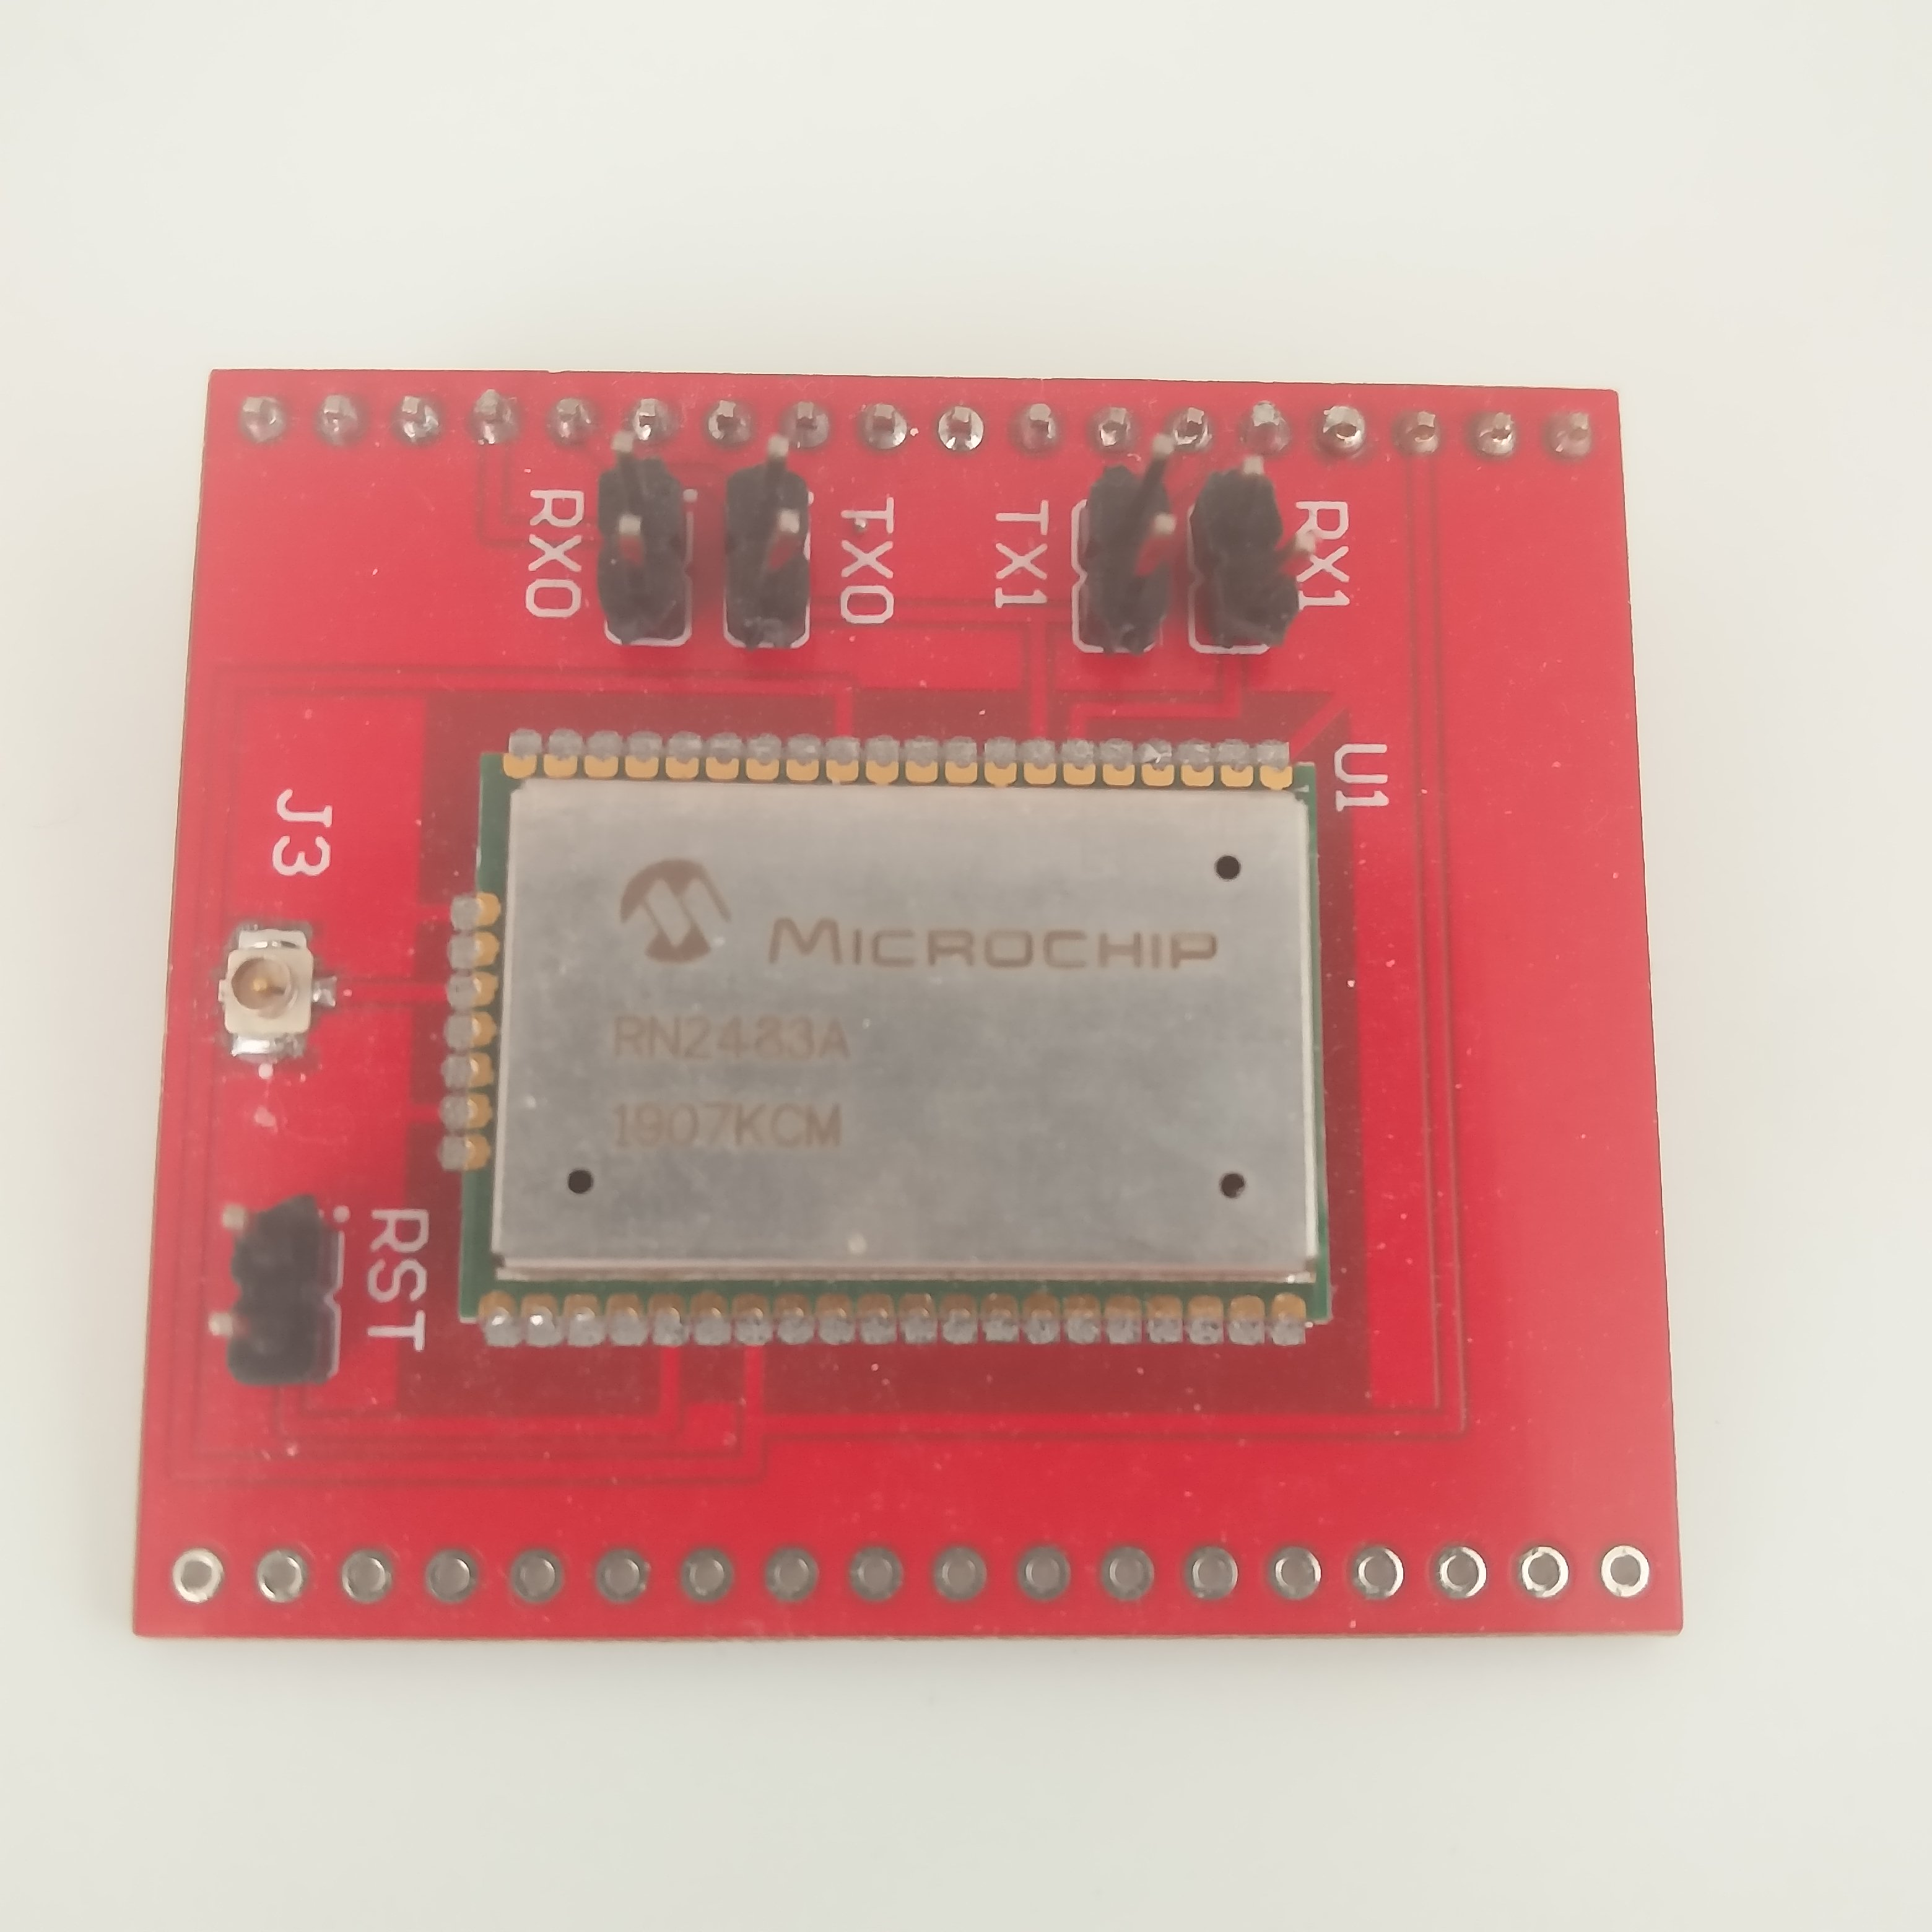
\includegraphics[width=0.9\textwidth]{presentation.tex/fig/rn2483.jpg}
    \caption{The RN2483 LoRa radio shield\label{fig:rn2483pic}}
\end{figure}
\end{column}
\begin{column}{0.4\textwidth}
\begin{figure}[H]
    \centering
    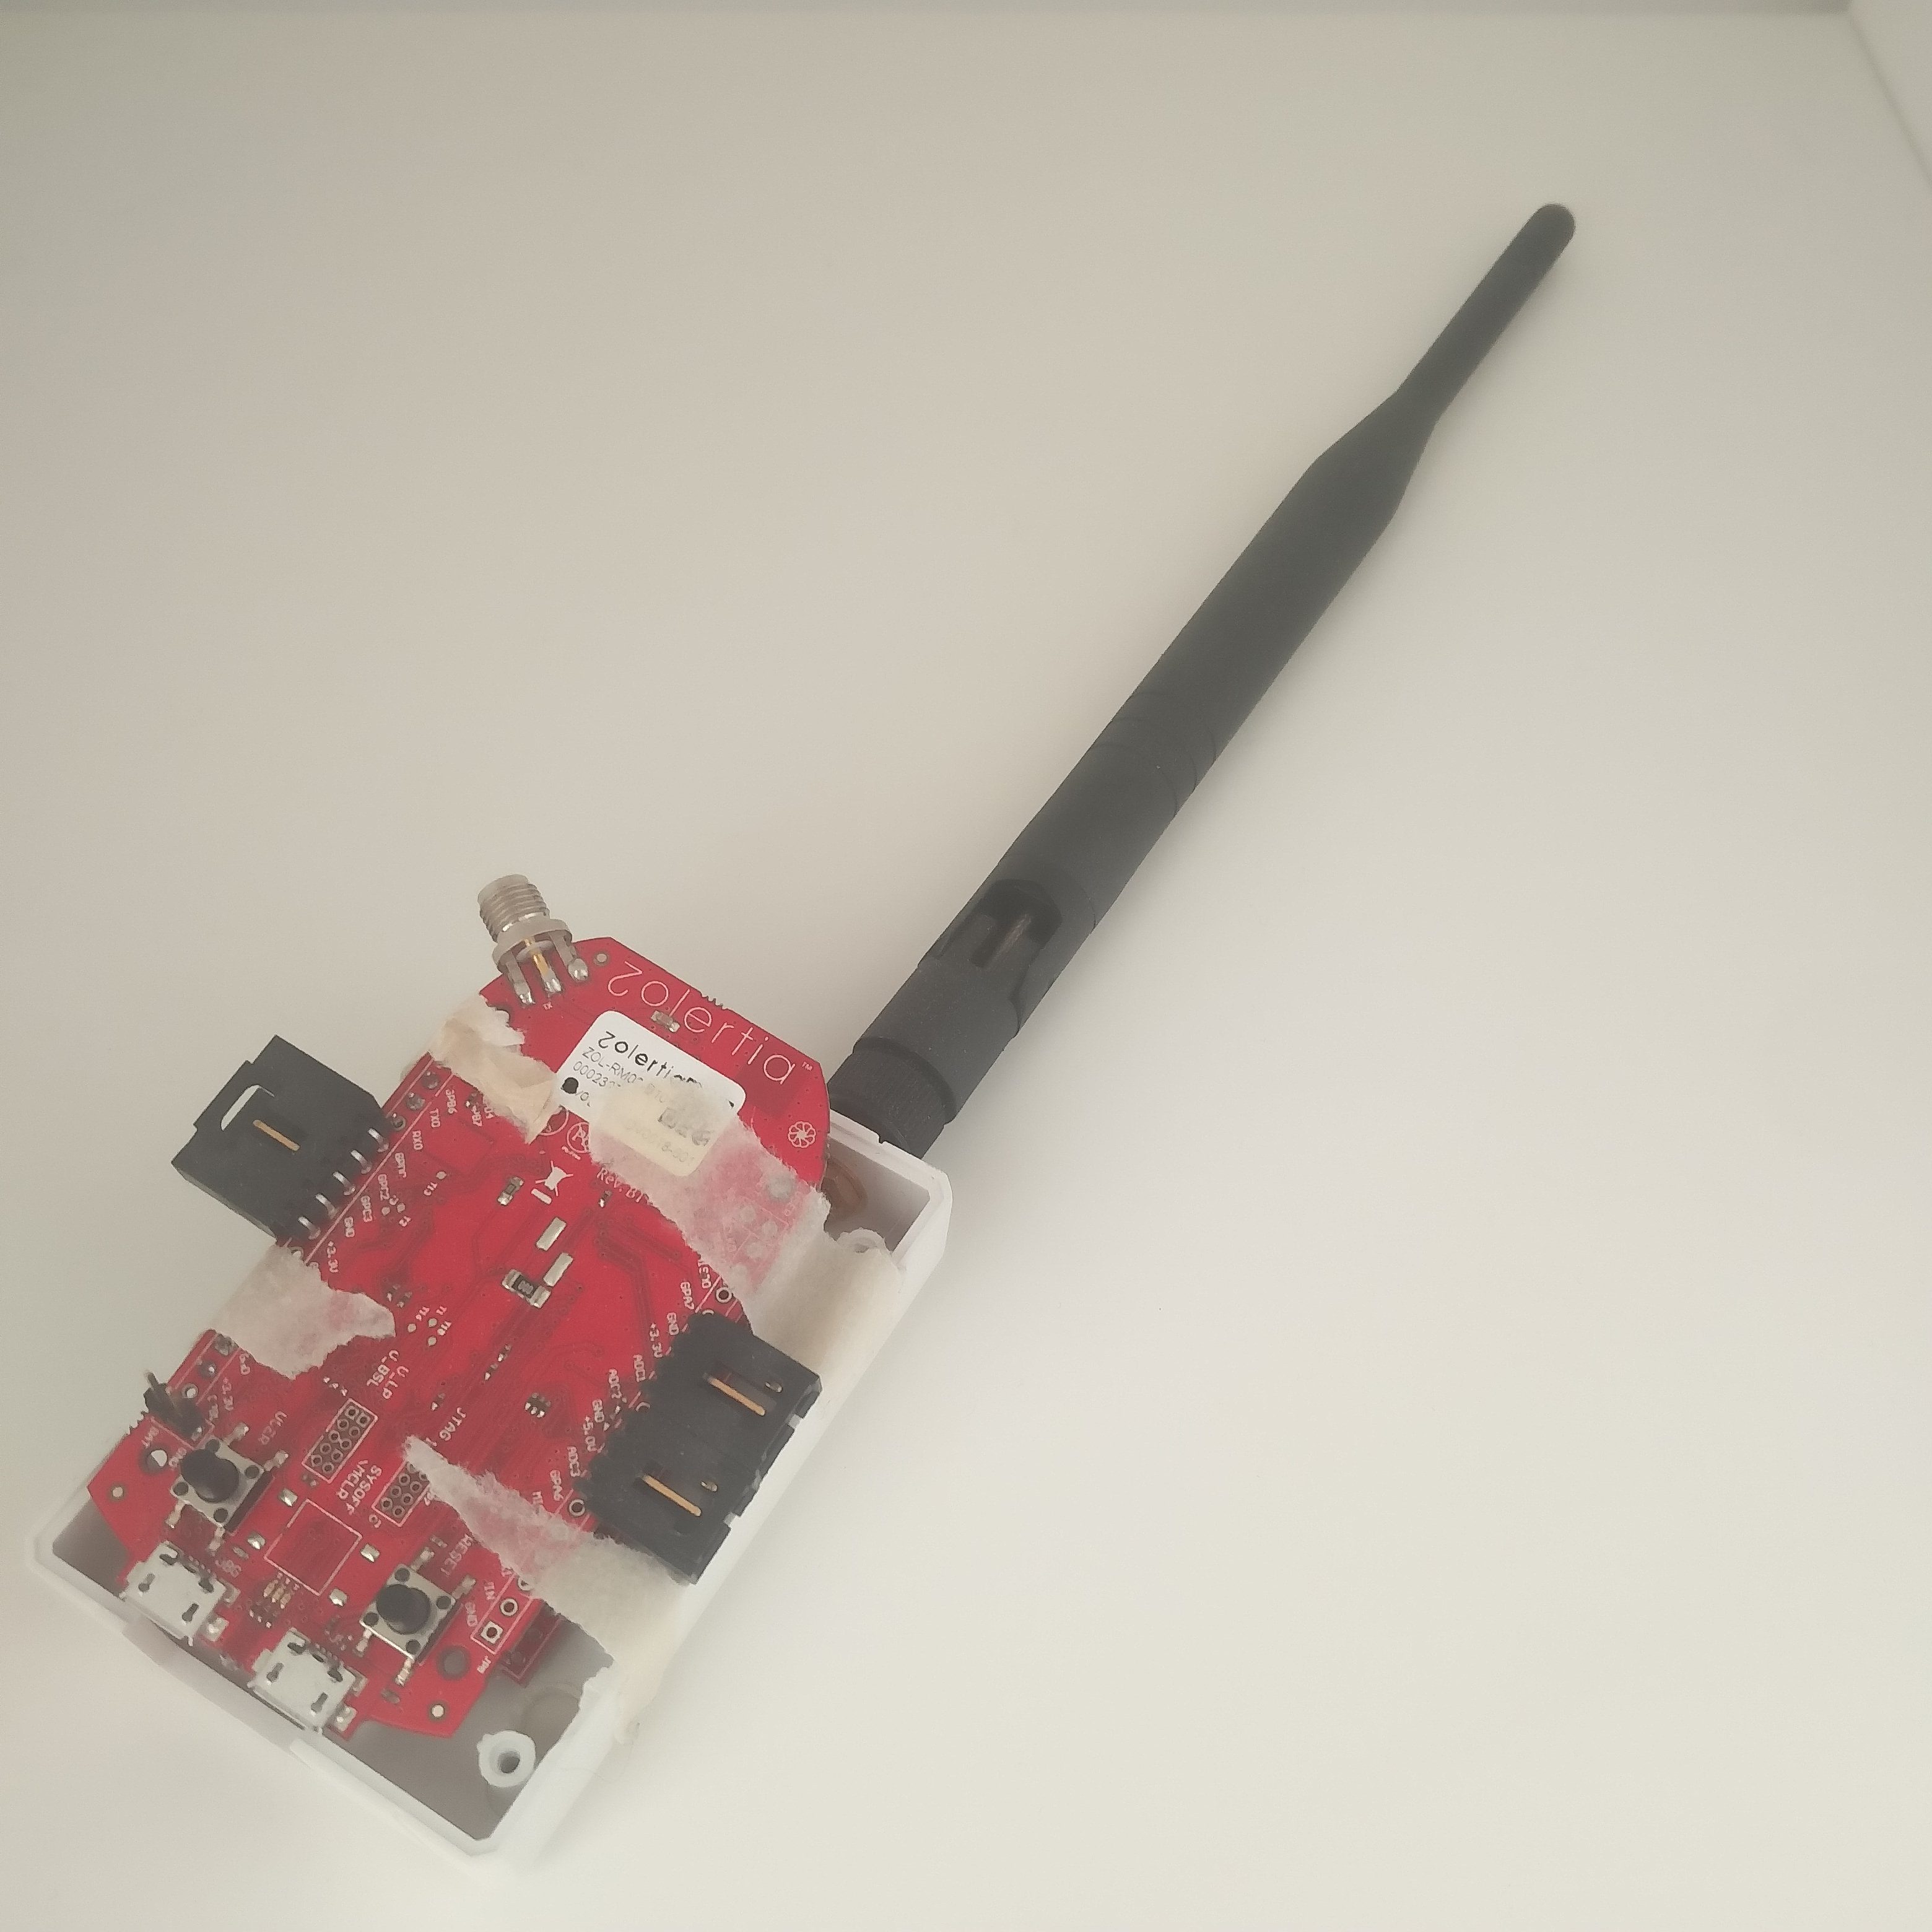
\includegraphics[width=0.9\textwidth]{presentation.tex/fig/zolertia.jpg}
    \caption{The Zolertia RE-Mote with the shield\label{fig:zolpic}}
\end{figure}
\end{column}
\begin{column}{0.2\textwidth}
\begin{figure}[H]
    \centering
    
\includegraphics[width=0.9\textwidth]{presentation.tex/fig/contiki.png}
    \caption{contiki-ng OS}
\end{figure}
\end{column}
\end{columns}
\end{frame}

\begin{frame}{Implementation}
\framesubtitle{Physical Layer: My Driver for LoRa Shield}

\begin{columns}
\begin{column}{0.5\textwidth}
\begin{itemize}
    \item Contiki Radio Driver
    \item Synchronized UART communications
\end{itemize}
\end{column}
\begin{column}{0.5\textwidth}
\begin{figure}[H]
\centering
\scalebox{0.8}{%
\begin{tikzpicture}[->,>=stealth',shorten >=1pt,auto,node distance=1.6cm]
\tikzstyle{comment}=[
  right=2pt,
  font=\small,
  fill=white,
  text=black,
  draw=black,
]

\tikzstyle{every state}=[rectangle,thick,
  draw=black,fill=gray!20,text=black,
  minimum width= 6cm,
  minimum height= 1.20cm
]

\tikzstyle{smallstate}=[rectangle,thick,
  draw=black,fill=gray!10,text=black,
  minimum width= 4cm,
  minimum height= 1.20cm
]

% \node[smallstate]         (A)                    {Network Layer};
% \node[smallstate]         (B) [below of=A]       {Routing};
% \begin{scope}[on background layer]
%   \node[state, fit=(A)(B)] (AB)                 {};
% \end{scope}
\node[state]         (AB)                    {};
\node[state]         (C) [below of=AB]       {};
\node[state]         (D) [below of=C]       {LoRa Driver};

\node[comment]       at (AB.north west) {Network Layer};
\node[comment]       at (C.north west) {MAC Layer};
\node[comment]       at (D.north west) {Physical Layer};
\end{tikzpicture}
}
\end{figure}
\end{column}
\end{columns}
\end{frame}

\begin{frame}{Implementation}
\framesubtitle{Medium Access Control with TSCH}

\begin{figure}[H]
\centering
\scalebox{0.8}{%
\begin{tikzpicture}[->,>=stealth',shorten >=1pt,auto,node distance=1.6cm]
\tikzstyle{comment}=[
  right=2pt,
  font=\small,
  fill=white,
  text=black,
  draw=black,
]

\tikzstyle{every state}=[rectangle,thick,
  draw=black,fill=gray!20,text=black,
  minimum width= 6cm,
  minimum height= 1.20cm
]

\tikzstyle{smallstate}=[rectangle,thick,
  draw=black,fill=gray!10,text=black,
  minimum width= 4cm,
  minimum height= 1.20cm
]

\node[state]         (AB)                    {};
\node[state]         (C) [below of=AB]       {TSCH};
\node[state]         (D) [below of=C]       {LoRa Driver};

\node[comment]       at (AB.north west) {Network Layer};
\node[comment]       at (C.north west) {MAC Layer};
\node[comment]       at (D.north west) {Physical Layer};
\end{tikzpicture}
}
\end{figure}
\end{frame}

\begin{frame}{Implementation}
\framesubtitle{My Adaptation of TSCH for LoRa}
\begin{columns}
\begin{column}{0.45\textwidth}
TSCH for LoRa adaptations
\begin{itemize}
    \item Time slot parts timing 
    \item Challenges
    \begin{itemize}
      \item $131 ms$ timing limit
      \item Interrupt clash
      \item Watchdog
   \end{itemize}
\end{itemize}
\end{column}
\begin{column}{0.55\textwidth}
\scalebox{0.45}{%
\begin{tikzpicture}[
  timeslot/.style={draw, rectangle, minimum size=1cm},
  description/.style={draw, rectangle, minimum size=1cm},
  arr/.style={help lines,black!70,<->},
]
\draw[arr,->] (-2, 1) -- node[fill=white] {$time$} (10, 1);
\foreach [evaluate={\ts=int(mod(\i, 4))}] \i in {0,...,7} {
  \node (ts\i) [timeslot] at (\i, 0) {$TS_{\ts}$};
}
\node (ts8) [minimum height=1cm, minimum width=2cm, black!70] at (8.5, 0) {\ldots};

\draw[help lines, black!70]
  (ts8.north west) -- (ts8.north east) node[fill=white, black!70] {$\ldots$};
\draw[help lines, black!70]
  (ts8.south west) -- (ts8.south east) node[fill=white, black!70] {$\ldots$};

\draw[ultra thick] 
  (ts0.south west) rectangle (ts3.north east)
  (ts4.south west) rectangle (ts7.north east);

\begin{scope}[xshift=-1.2cm,yshift=-2cm,inner sep=0pt, outer sep=0pt]
  \node (desc) [fit={(-1.5,0) (0,1)}, label=center:{TX}] {};
  \node (desc0) [description, fit={(0,0) (3,1)}, label=center:{tx\_offset}] {};
  \node (desc1) [description, fit={(3,0) (6,1)}, label=center:{max\_tx}] {};
  \node (desc2) [description, fit={(6,0) (9,1)}, label=center:{rx\_ack\_delay}] {};
  \node (desc3) [description, fit={(9,0) (12,1)}, label=center:{max\_ack}] {};
\end{scope}

\draw[help lines, black!70,-]
  ([yshift=0pt]ts4.south west) -- 
  ([yshift=0pt]{desc0.north west});
\draw[help lines, black!70,-]
  ([yshift=0pt]ts4.south east) -- 
  ([yshift=0pt]{desc3.north east});

\begin{scope}[xshift=-1.2cm,yshift=-3.5cm,inner sep=0pt, outer sep=0pt]
  \node (ddesc) [fit={(-1.5,0) (0,1)}, label=center:{RX}] {};
  \node (ddesc0) [description, fit={(0,0) (3,1)}, label=center:{rx\_offset}] {};
  \node (ddesc1) [description, fit={(3,0) (6,1)}, label=center:{rx\_wait}] {};
  \node (ddesc2) [description, fit={(6,0) (9,1)}, label=center:{tx\_ack\_delay}] {};
  \node (ddesc3) [description, fit={(9,0) (12,1)}, label=center:{max\_ack}] {};
\end{scope}

\draw[help lines, black!70,-]
  ([yshift=0pt]desc0.south west) -- 
  ([yshift=0pt]{ddesc0.north west});
\draw[help lines, black!70,-]
  ([yshift=0pt]desc3.south east) -- 
  ([yshift=0pt]{ddesc3.north east});
\end{tikzpicture}
}

\end{column}
\end{columns}
\end{frame}

\begin{frame}{Implementation}
\framesubtitle{My Adaptation of TSCH for LoRa}
\begin{columns}
\begin{column}{0.5\textwidth}
Hardware specific issues
\begin{itemize}
    \item Physical delay of RN2483
    \only<2->{
      \item No reception ack
      % \begin{itemize}
      %   \item Less precision
      % \end{itemize}
    }
\end{itemize}
\end{column}
\begin{column}{0.5\textwidth}

\resizebox{5.2cm}{3.4cm}{%
\begin{tikzpicture}[
  timeslot/.style={draw, rectangle, minimum size=1cm},
  description/.style={draw, rectangle, minimum size=1cm},
  arr/.style={help lines,black!70,<->},
]
\draw[arr,->] (-1.5, 1) -- node[fill=white] {$time$} (6, 1);
\foreach [evaluate={\ts=int(mod(\i, 4))}] \i in {0,...,3} {
  \node (ts\i) [timeslot] at (\i, 0) {$TS_{\ts}$};
}
\node (ts4) [minimum height=1cm, minimum width=2cm, black!70] at (4.5, 0) {\ldots};
\draw[help lines, black!70]
  (ts4.north west) -- (ts4.north east) node[fill=white, black!70] {$\ldots$};
\draw[help lines, black!70]
  (ts4.south west) -- (ts4.south east) node[fill=white, black!70] {$\ldots$};

\draw[ultra thick] 
  (ts0.south west) rectangle (ts3.north east);

\begin{scope}[xshift=-1.2cm,yshift=-2.5cm,inner sep=0pt, outer sep=0pt]
  \node (desc) [draw,rectangle,fit={(0,0) (6,1)}, label=left:{Transmitter~}] {};
  \node (desc1) [description, fill=orange!20, fit={(3,0) (6,1)}, label=center:{data}] {};
  \node (desc0) [description, fill=gray!20, fit={(1,0) (3,1)}, label=center:{tx\_offset}] {};
  \node (desccont) [black!70, fit={(6,0) (8,1)}] {\ldots};
  \draw[help lines, black!70]
    (desccont.north west) -- (desccont.north east) node[fill=white, black!70] {$\ldots$};
  \draw[help lines, black!70]
    (desccont.south west) -- (desccont.south east) node[fill=white, black!70] {$\ldots$};
  \only<1>{
    \draw[pattern=north west lines, pattern color=green!50] (2.6,0) rectangle (3,1);
  }
\end{scope}

\begin{scope}[xshift=-1.2cm,yshift=-4.5cm,inner sep=0pt, outer sep=0pt]
  \node (ddesc) [draw,rectangle,fit={(0,0) (6,1)}, label=left:{Receiver~}] {};
  \node (ddesc0) [description, fill=gray!20, fit={(1,0) (3,1)}, label=center:{rx\_offset}] {};
  \draw[pattern=north west lines, pattern color=orange!50] (3,0) rectangle (6,1);
  \node (ddesccont) [black!70, fit={(6,0) (8,1)}] {\ldots};
  \draw[help lines, black!70]
    (ddesccont.north west) -- (ddesccont.north east) node[fill=white, black!70] {$\ldots$};
  \draw[help lines, black!70]
    (ddesccont.south west) -- (ddesccont.south east) node[fill=white, black!70] {$\ldots$};
  \only<1>{
    \draw[pattern=north west lines, pattern color=green!50] (6,0) rectangle (6.4,1);
  }
\end{scope}

\only<1->{
\begin{scope}[xshift=-1.2cm,yshift=-6.5cm,inner sep=0pt, outer sep=0pt]
  \node (comment) [red!70, fit={(5,0) (7,1)}] {};
\end{scope}
}

\only<2->{
\begin{scope}[xshift=-1.2cm,yshift=-6.5cm,inner sep=0pt, outer sep=0pt]
  \node (comment) [red!70, fit={(5,0) (7,1)}] {No Ack};
  \draw[help lines, thick, red!70,->]
    ([yshift=0pt]{comment.north west}) --
    ([yshift=0pt]ddesc0.south east);
\end{scope}
}

\draw[help lines, black!70,-]
  (ts3.south west) -- 
  ({desc.north west});
\draw[help lines, black!70,-]
  (ts3.south east) -- 
  ([xshift=12pt]{desccont.north east});
\end{tikzpicture}
}
\end{column}
\end{columns}
\end{frame}

% \begin{frame}{Validation}
% \framesubtitle{Driver}
% \begin{columns}
% \begin{column}{0.5\textwidth}
% \begin{itemize}
%     \item Validate the LoRa Driver
%     \item Ping-Pong example
%     \item Driver controlled by MAC layer
%     \begin{itemize}
%       \item Fully working on Contiki
%     \end{itemize}
% \end{itemize}
% \end{column}
% \begin{column}{0.5\textwidth}
% \begin{figure}[H]
% \centering
% \begin{sequencediagram}
% \newthread{A}{Mote A}{}
% \newinst[1]{B}{Mote B}{}

% \begin{call}[4]{A}{ping}{B}{pong}
% \end{call}
% \end{sequencediagram}
% \end{figure}
% \end{column}
% \end{columns}
% \end{frame}

\begin{frame}{Validation}
\framesubtitle{Testing Multi-hop Routing Protocol with LoRa}
\begin{columns}
\begin{column}{0.5\textwidth}
\begin{itemize}
  \item Using the complete stack
  % \item Testing channel hopping
  \item Testing with custom schedule
\end{itemize}
\end{column}
\begin{column}{0.5\textwidth}
\begin{figure}[H]
\centering
\scalebox{0.8}{%
\begin{tikzpicture}[->,>=stealth',shorten >=1pt,auto,node distance=1.6cm]
  \tikzstyle{comment}=[ right=2pt, font=\small, fill=white, text=black, draw=black, ]
  \tikzstyle{every state}=[rectangle,thick, draw=black,fill=gray!20,text=black, minimum width= 6cm, minimum height= 1.20cm ]
  \tikzstyle{smallstate}=[rectangle,thick, draw=black,fill=gray!10,text=black, minimum width= 4cm, minimum height= 1.20cm ]
  % \node[state]              (T)                    {UDP};
  \node[smallstate]         (A)        {IPv6};
  \node[smallstate]         (B) [below of=A]       {RPL};
  \begin{scope}[on background layer]
    \node[state, fit=(A)(B)] (AB)                 {};
  \end{scope}
  \node[state,below=1cm]         (C) [below of=AB]       {TSCH};
  \node[state]         (D) [below of=C]       {LoRa};
  % \node[comment]       at (T.north west) {Transport Layer};
  \node[comment]       at (AB.north west) {Network Layer};
  \node[comment]       at (C.north west) {MAC Layer};
  \node[comment]       at (D.north west) {Physical Layer};
\end{tikzpicture}
}
\caption{Packet route over my custom schedule}
\end{figure}
\end{column}
\end{columns}
\end{frame}

\begin{frame}{Validation}
\framesubtitle{Choose minimum schedule}
\begin{figure}[H]
    \centering
    \resizebox{9.4cm}{4.5cm}{
  \begin{tikzpicture}[]

  \begin{scope}[
      xshift=-0.2cm,
      asn/.style={black!70, minimum width=2cm},
      timeslot/.style={draw, rectangle, minimum width=2cm, minimum height=1cm},
      arr/.style={help lines,black!70,<->},
  ]
    \draw[arr,->] (-1, 2) -- node[fill=white] {$time$} (15, 2);
    \foreach \i in {0,...,7} {
      \node (ts\i) [asn] at (2*\i, 1) {$TS_{\i}$};
    }
    \node (tss0) [timeslot] at (0, 0) {\tiny Shared};
    \node (tss1) [timeslot] at (2, 0) {\tiny B $\rightarrow$ A};
    \node (tss2) [timeslot] at (4, 0) {\tiny C $\rightarrow$ A};
    \node (tss3) [timeslot] at (6, 0) {\tiny C $\rightarrow$ B};
    \node (tss4) [timeslot] at (8, 0) {\tiny A $\rightarrow$ C};
    \node (tss5) [timeslot] at (10, 0) {\tiny D $\rightarrow$ B};
    \node (tss6) [timeslot] at (12, 0) {\tiny B $\rightarrow$ D};
    \node (tss7) [timeslot, fill=black!30] at (14, 0) {};
  \end{scope}
  \begin{scope}[xshift=7.2cm,yshift=-2cm,->,>=stealth',shorten >=1pt,auto,node distance=2.5cm]
    \tikzstyle{every state}=[thick,draw=gray!50,fill=gray!20,draw=none,text=black]

    \node[state,thick,draw=red!40]         (A) [] {A};
    \node[state]         (B) [below of=A]       {B};
    \node[state]         (C) [right of=B]       {C};
    \node[state]         (D) [left of=B]       {D};

    \path (A) edge [bend left,color=red!70] node {$TS_4$} (C)
          (B) edge [bend left,color=red!70] node {$TS_1$} (A)
              edge [bend left] node {$TS_6$} (D)
          (C) edge [bend left] node[above right] {$TS_2$} (A)
              edge [bend left] node {$TS_3$} (B)
          (D) edge [bend left, color=red!70] node {$TS_5$} (B);
  \end{scope}
\end{tikzpicture}
}
\end{figure}
\end{frame}

\begin{frame}{Validation}
\framesubtitle{Testing Robustness to Channel Jamming}
\begin{figure}[H]
\centering

\begin{tikzpicture}[auto, node distance=2cm,>=latex']

\tikzset{
  block/.style = {draw, fill=white, rectangle, minimum height=3em, minimum width=2cm},
  input/.style = {coordinate},
  output/.style = {coordinate},
  pinstyle/.style = {pin edge={to-,t,black}},
  radiation/.style={decorate,decoration={expanding waves,angle=12,segment length=4pt}},
  zigzag/.style={to path={ -- ($(\tikztostart)!.55!-7:(\tikztotarget)$) -- ($(\tikztostart)!.45!7:(\tikztotarget)$) -- (\tikztotarget) \tikztonodes}}
}
\node[block](tx){Transmitter Node};
\node[block,above right= 2cm of tx](ttx){Jammer};
\node[block,right = 5cm of tx](rx){Receiver Node};

\draw[radiation] ([shift={(1cm,0cm)}]tx.east)-- node [above=5mm] {} ([shift={(-1cm,0cm)}]rx.west);
\draw[-stealth,line width=1mm] (ttx.south) to[zigzag] +(0,-1.5);
\end{tikzpicture}
\caption{Testing setup}
\end{figure}
\end{frame}

\begin{frame}{Validation}
\framesubtitle{Testing Robustness to Channel Jamming}
\begin{figure}[H]
  \centering
  \scalebox{0.8}{%
  \begin{tikzpicture}[
    asn/.style={black!70, minimum size=1cm},
    timeslot/.style={draw, rectangle, minimum size=1cm},
    arr/.style={help lines,black!70,<->},
    desc/.style={black!70},
  ]
    \foreach [evaluate={\ts=int(mod(\i, 4))}] \i in {0,...,11} {
    \node (3ts\i) [timeslot] at (\i, 3) {};
    }
    \foreach [evaluate={\ts=int(mod(\i, 4))}] \i in {0,...,11} {
    \node (2ts\i) [timeslot] at (\i, 2) {};
    }
    \foreach [evaluate={\ts=int(mod(\i, 4))}] \i in {0,...,11} {
    \node (1ts\i) [timeslot] at (\i, 1) {};
    }
    \foreach [evaluate={\ts=int(mod(\i, 4))}] \i in {0,...,11} {
    \node (0ts\i) [asn] at (\i, 0) {$TS_{\ts}$};
    }

    \node (choff3) [black!70] at (-1.0, 3) {$Ch_2$};
    \node (choff2) [black!70] at (-1.0, 2) {$Ch_1$};
    \node (choff1) [black!70] at (-1.0, 1) {$Ch_0$};

    \begin{scope}[on background layer]
    \fill[blue!50] (3ts8.south west) rectangle (3ts8.north east);
    \fill[blue!50] (2ts4.south west) rectangle (2ts4.north east);
    \fill[blue!50] (1ts0.south west) rectangle (1ts0.north east);
    \end{scope}

    \draw[ultra thick]
        (1ts0.south west) rectangle (3ts3.north east)
        (1ts4.south west) rectangle (3ts7.north east)
        (1ts8.south west) rectangle (3ts11.north east);
    \draw[arr,->] ([yshift=-10pt]0ts0.south west) -- node[fill=white] {$time$} ([yshift=-10pt]{0ts11.south east});

    \draw[pattern=north west lines, pattern color=red!90] (1ts0.north west) rectangle (1ts11.south east);
  \end{tikzpicture}
  }
\caption{Channel Hopping sequence with single jammed channel}
\end{figure}
\end{frame}

% \begin{frame}{Validation}
% \framesubtitle{Jamming}
% \begin{figure}[H]
%   \centering
%   \begin{tikzpicture}

%   \begin{groupplot}[group style={group size=1 by 2,
%       horizontal sep=0pt,
%       vertical sep=1cm},
%       height=6cm,width=6cm,
%   ]
%   \nextgroupplot[
%     ycomb,
%     width=0.8\textwidth,
%     height=0.25\textwidth,
%     axis lines=middle,
%     ymin=0,
%     ymax=4,
%     ylabel={$Retry_{number}$},
%     ylabel near ticks,
%     yticklabel style={/pgf/number format/1000 sep=},
%     xmin=0,
%     xmax=50,
%     xlabel={$Transmission_{number}$},
%     xlabel near ticks,
%   ]
%     \addplot[color=blue, mark=x] coordinates {
%       (1,1)
%       (2,2)
%       (3,0)
%       (4,0)
%       (5,0)
%       (6,1)
%       (7,0)
%       (8,0)
%       (9,1)
%       (10,0)
%       (11,1)
%       (12,1)
%       (13,2)
%       (14,0)
%       (15,2)
%       (16,0)
%       (17,1)
%       (18,1)
%       (19,1)
%       (20,0)
%       (21,4)
%       (22,0)
%       (23,0)
%       (24,1)
%       (25,0)
%       (26,0)
%       (27,2)
%       (28,1)
%       (29,0)
%       (30,0)
%       (31,1)
%       (32,1)
%       (33,0)
%       (34,0)
%       (35,0)
%       (36,1)
%       (37,2)
%       (38,0)
%       (39,0)
%       (40,0)
%       (41,1)
%       (42,1)
%       (43,0)
%       (44,0)
%       (45,3)
%       (46,1)
%       (47,0)
%       (48,0)
%       (49,1)
%       (50,1)
%     };
%   \end{groupplot}
%   \end{tikzpicture}
%   % \caption{Retransmission per packet\label{fig:retransmission}}
% \end{figure}
% \end{frame}
